\documentclass[letter,12pt]{article}
\usepackage[paperheight=27.94cm,paperwidth=21.59cm,bindingoffset=0in,left=3cm,right=2.0cm, top=3.5cm,bottom=2.5cm, headheight=200pt, headsep=1.0\baselineskip]{geometry}
\usepackage{graphicx,lastpage}
\usepackage{upgreek}
\usepackage{censor}
\usepackage[spanish,es-tabla]{babel}
\usepackage{pdfpages}
\usepackage{tabularx}
\usepackage{graphicx}
\usepackage{adjustbox}
\usepackage{xcolor}
\usepackage{colortbl}
\usepackage{rotating}
\usepackage{multirow}
\usepackage[utf8]{inputenc}
\usepackage{float}
\usepackage{hyperref}
\usepackage[utf8]{inputenc}
\usepackage[T1]{fontenc}

\renewcommand{\tablename}{Tabla}
\usepackage{fancyhdr}
\pagestyle{fancy}
\usepackage{listings}
\usepackage{caption}

\definecolor{darkerGreen}{rgb}{0.0, 0.5, 0.0}


% Define counter for code listings


\newcounter{codecount}
\renewcommand{\thecodecount}{\arabic{codecount}}

% Redefine caption for listings
\DeclareCaptionFormat{myformat}{Código \thecodecount: #3}
\captionsetup[lstlisting]{format=myformat, labelformat=empty}

\lstdefinelanguage{JavaScript}{
  keywords={break, case, catch, continue, debugger, default, delete, do, else, finally, for, function, if, in, instanceof, new, return, switch, this, throw, try, typeof, var, void, while, with, let, const, of},
  keywordstyle=\color{blue}\bfseries,
  ndkeywords={class, export, boolean, throw, implements, import, this},
  ndkeywordstyle=\color{blue}\bfseries,
  identifierstyle=\color{black},
  sensitive=false,
  comment=[l]{//},
  morecomment=[s]{/*}{*/},
  commentstyle=\color{darkerGreen}\ttfamily,
  stringstyle=\color{red}\ttfamily,
  morestring=[b]',
  morestring=[b]"
}

\lstdefinestyle{mystyle}{
  language=JavaScript,
  basicstyle=\ttfamily\small,
  backgroundcolor=\color[rgb]{0.95, 0.95, 0.95},
  numberstyle=\tiny\color{gray},
  numbersep=5pt,
  stepnumber=1,
  frame=single,
  breaklines=true,
  showstringspaces=false,
  captionpos=b,
  numbers=left,
escapeinside={\%*}{*)},
  morekeywords={*,...},
  postbreak=\mbox{\textcolor{cyan}{$\hookrightarrow$}\space}  
}



\lstset{style=mystyle}




%
\begin{document}
%
   \title{\Huge{Informe Laboratorio 4}}

   \author{\textbf{Sección 1} \\  \\Alumno Omar Marca \\ e-mail: omar.marca@mail.udp.cl}
          
   \date{Mayo de 2024}

   \maketitle
   
   \tableofcontents
 
  \newpage
  

\section{Descripción de actividades}
Para este laboratorio, deberá utilizar Tampermonkey y la librería CryptoJS (con SRI) para lograr obtener los mensajes que le está comunicando su informante. En esta ocasión, su informante fue más osado y se comunicó con usted a través de un sitio web abierto a todo el público https://cripto.tiiny.site/.\par
Sólo un ojo entrenado como el suyo logrará descifrar cuál es el algoritmo de cifrado utilizado y cuál es la contraseña utilizada para lograr obtener la información que está oculta.
\begin{enumerate}
    \item Desarrolle un plugin para tampermonkey que permita obtener la llave para el descifrado de los mensajes ocultos en la página web. La llave debe ser impresa por la consola de su navegador al momento de cargar el sitio web. Utilizar la siguiente estructura:
    \begin{itemize}
        \item   La llave es: KEY
    \end{itemize}
    
    \item En el mismo plugin, se debe detectar el patrón que permite identificar la cantidad de mensajes cifrados. Debe imprimir por la consola la cantidad de mensajes cifrados. Utilizar la siguiente estructura:
    Los mensajes cifrados son: NUMBER
    
    \item En el mismo plugin debe obtener cada mensaje cifrado y descifrarlo. Ambos mensajes deben ser informados por la consola (cifrado espacio descifrado) y además cada mensaje en texto plano debe ser impreso en la página web. \par
    El script desarrollado debe ser capaz de obtener toda la información del sitio web (llave, cantidad de mensajes, mensajes cifrados) sin ningún valor forzado. Para verificar el correcto funcionamiento de su script se utilizará un sitio web con otro texto y una cantidad distinta de mensajes cifrados. Deberá indicar la url donde se podrá descargar su script.\par
    Un ejemplo de lo que se debe visualizar en la consola, al ejecutar automáticamente el script, es lo siguiente:

\clearpage

    \begin{figure}[H]
        \centering
        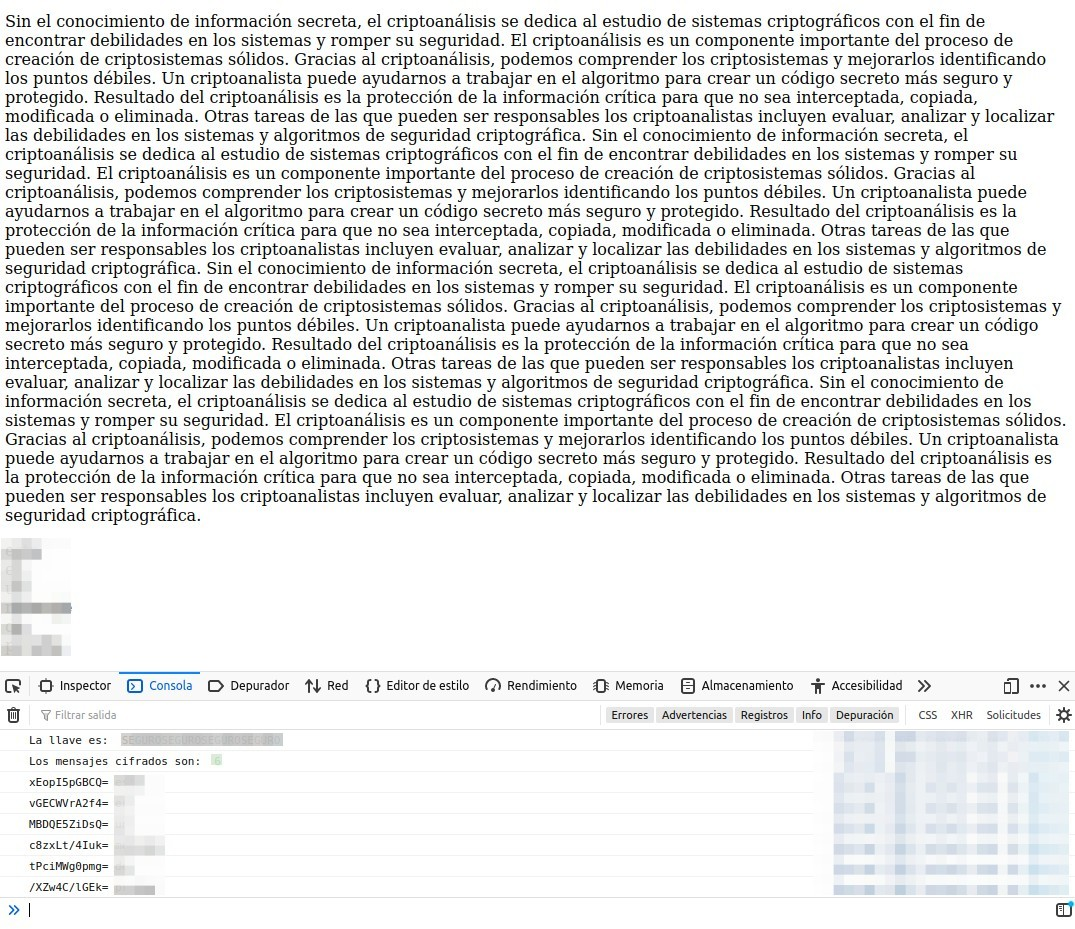
\includegraphics[width=16cm]{Images/ejemplo.jpg}
        \label{fig:ejemplo}
    \end{figure}
    
\clearpage

\end{enumerate}



\section{Desarrollo (Parte 1)}
\subsection{Detecta el cifrado utilizado por el informante}

Al cargar la página entregada por el informante se muestra un texto plano que no entrega información ni algún patrón que pueda sugerir un mensaje secreto. No obstante si se abre el inspector de la página, se puede apreciar que además del componente del texto, hay 6 componentes ``div" sospechosos que contienen un mensaje en su id y una clase con numeros secuenciales tal y como se muestra en la figura \ref{fig:Cifradodelinformante}:

\begin{figure}[H]
    \centering
    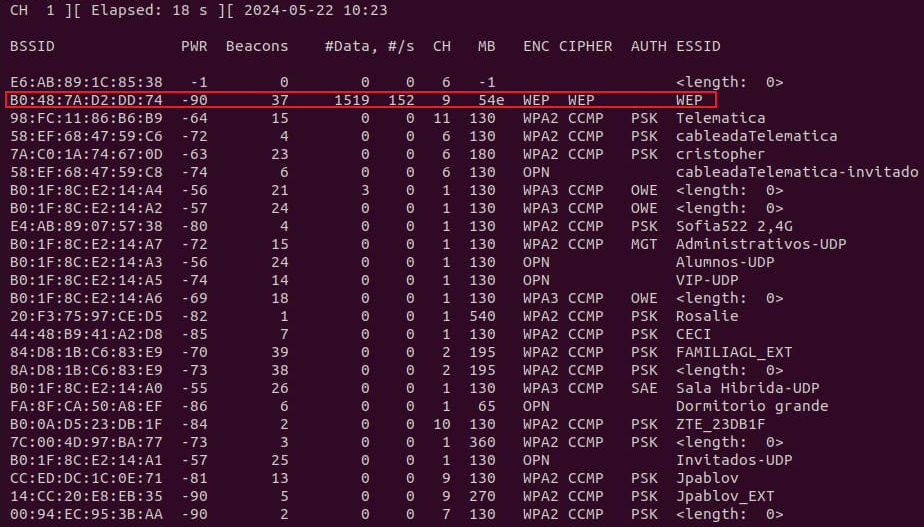
\includegraphics[width=0.7\textwidth]{Images/Parte1/2.1.png}
    \caption{Cifrado del informante}
    \label{fig:Cifradodelinformante}
\end{figure}

Para saber el contenido de este mensaje cifrado, se hace uso de la extensión de navegador de Tampermonkey.

\clearpage

\subsection{Logra que el script solo se gatille en el sitio usado por el informante}

Para realizar el Script en Tampermonkey, se hará uso del código proporcionado en la página de Greasy Fork por el usuario \href{https://greasyfork.org/es/users/1214768-akumukernel}{AkumuKernel} en \href{https://greasyfork.org/es/scripts/479454-cryptojs/code}{este enlace}. A continuación se hará explicación del código:\\
\\
Para que el Script de Tampermonkey solo se engatille en la página web usada por el informante, se debe colocar ``@match'' seguido de la dirección de la página web del informante en el apartado de ``==UserScript=='' al principio del código. A continuación se muestra como se debe escribir la sintaxis a seguir en el código \ref{code:ScriptGatilla}:\\

\refstepcounter{codecount}\label{code:ScriptGatilla}
\begin{lstlisting}[caption=Apuntar a la página donde se debe ejecutar, label=lst:javascript_example]
// ==UserScript==

  // @match        https://cripto.tiiny.site/
  
// ==/UserScript==

\end{lstlisting}




\clearpage

\subsection{Define función que obtiene automáticamente el password del documento}

Desglosando el código obtenido en la pagina de \href{https://greasyfork.org/es/scripts/479454-cryptojs/code}{Greasy Fork}, se obtiene la primera parte para obtener la password del documento en el fragmento de código \ref{code:ObtenerPasswordDocumento} 

\refstepcounter{codecount}\label{code:ObtenerPasswordDocumento}
\begin{lstlisting}[caption= Función para obtener la password del documento , label=lst:javascript_example]
    (function() {
     'use strict';
     var CryptoJS = window.CryptoJS;
     // Parte 1

     var parrafoDiv = document.querySelector('p');
     if (!parrafoDiv) return;

     var textoCompleto = parrafoDiv.innerText;
     var oraciones = textoCompleto.split('. ');
     var contrasena = "";
     for (var i = 0; i < oraciones.length; i++) {
         var primeraLetra = oraciones[i].charAt(0);
         contrasena += primeraLetra;
     }

     if (contrasena.length > 24) {
         contrasena = contrasena.substring(0, 24);
     }

     console.log("La llave es:", contrasena);
})();

\end{lstlisting}

Básicamente lo que hace este fragmento de código \ref{code:ObtenerPasswordDocumento} es buscar un patrón de repetición de la página del informante para encontrar la contraseña. Para ello se tiene lo siguiente:

\begin{enumerate}
    \item Línea 6: Obtiene componente del párrafo mediante la etiqueta ``p''.

    \item Línea 10: Separa las oraciones del texto por puntos seguidos.

    \item Línea 12-15: Itera sobre la primera letra de cada oración para concatenarlas en una variable.

    \item Línea 17-19: Si el largo de la contraseña es mayor a 24, se trunca.

    \item Línea 21: Se imprime la contraseña encontrada.
\end{enumerate}

\clearpage

\subsection{Muestra la llave por consola}

Una vez guardado el código del punto 2.3, se recarga la página y se obtiene la clave tal y como se muestra en la figura \ref{fig:2.4}

\begin{figure}[H]
    \centering
    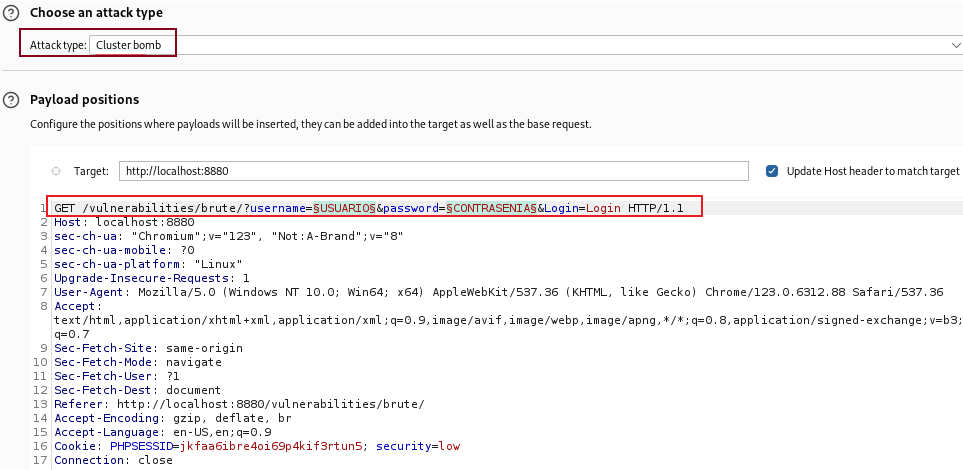
\includegraphics[width=0.9\textwidth]{Images/Parte1/2.4.png}
    \caption{Obtención de la llave por consola}
    \label{fig:2.4}
\end{figure}

Como se puede apreciar, la clave es ``SEGUROSEGUROSEGUROSEGURO'' la cual es señalada por una flecha roja.

\clearpage

\section{Desarrollo (Parte 2)}

\subsection{Reconoce automáticamente la cantidad de mensajes cifrados}

Si bien, se sabe que en el inspector se muestran 6 mensajes, para que mediante un script se sepa la cantidad de mensajes cifrados, se debe reconocer que estos mensajes tienen un patrón con el cual se pueden identificar su repetición. Entonces, a continuación se muestra en el fragmento de código \ref{code:CantidadDeMensajesCifrados} extraído de la página de \href{https://greasyfork.org/es/scripts/479454-cryptojs/code}{Greasy Fork}, la forma en que se obtiene el numero de mensajes cifrados: \\

\refstepcounter{codecount}\label{code:CantidadDeMensajesCifrados}
\begin{lstlisting}[caption= Muestra la cantidad de mensajes cifrados, label=lst:javascript_example]
 // Parte 2
 var elementos = document.querySelectorAll('div[class^="M"]');

 var repeticiones = {};
 var patron = /\d+/;

 for (i = 0; i < elementos.length; i++) {
     var clases = elementos[i].classList;
     for (var j = 0; j < clases.length; j++) {
         var clase = clases[j];
         if (patron.test(clase)) {
             if (repeticiones[clase]) {
                 repeticiones[clase]++;
             } else {
                 repeticiones[clase] = 1;
             }
         }
     }
 }

 var mensajeCifrado = "Los mensajes cifrados son: " + Object.keys(repeticiones).length;
 console.log(mensajeCifrado);

\end{lstlisting}

\begin{enumerate}
    \item Línea 2: Devuelve una lista de componentes asociados al a expresión regular ``div[class\^ ="M"]''

    \item Línea 7-19: Cuenta las veces que se repiten los mensajes según la expresión regular declarada en la línea 2 y 5 de tal forma que se guardan las veces que se repite un mensaje. Además, estas concurrencias se guardan en la variable ``repeticiones'' declarada en la línea 4. Es decir, este bloque de código es el que hace el conteo de la cantidad de mensajes cifrados.

    \item Línea 21-22: Le da formato al mensaje e imprime por consola.
    
\end{enumerate}

\clearpage

\subsection{Muestra la cantidad de mensajes por consola}

Al concatenar el código de la parte 1 con el de la sección 3.1, se debe guardar en Tampermonkey y luego Recargar la página. Entonces, al revisar la consola, se puede ver la cantidad de mensajes cifrados tal y como se puede ver en la figura \ref{fig:Cantidaddemensajesmostradosporconsola}:

\begin{figure}[H]
    \centering
    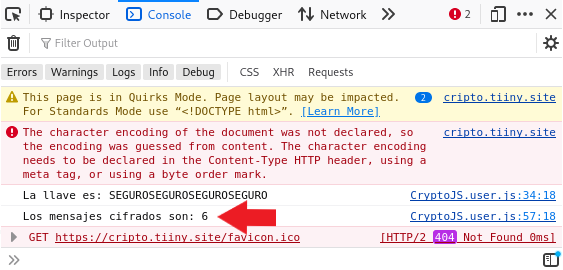
\includegraphics[width=0.9\textwidth]{Images/Parte2/3.2.png}
    \caption{Cantidad de mensajes mostrados por consola}
    \label{fig:Cantidaddemensajesmostradosporconsola}
\end{figure}

La cantidad de mensajes son 6 y se encuentran señalados mediante una flecha roja.

\clearpage

\section{Desarrollo (Parte 3)}

\subsection{Importa la librería cryptoJS}

Para importar la librería de CryptoJS se debe acceder al sitio web de \href{https://cdnjs.com/libraries/crypto-js}{cdnjs en este enlace} que mostrará la URL para importar la librería tal y como se puede ver en el siguiente figura \ref{fig:libreriadeCryptoJS}:

\begin{figure}[H]
    \centering
    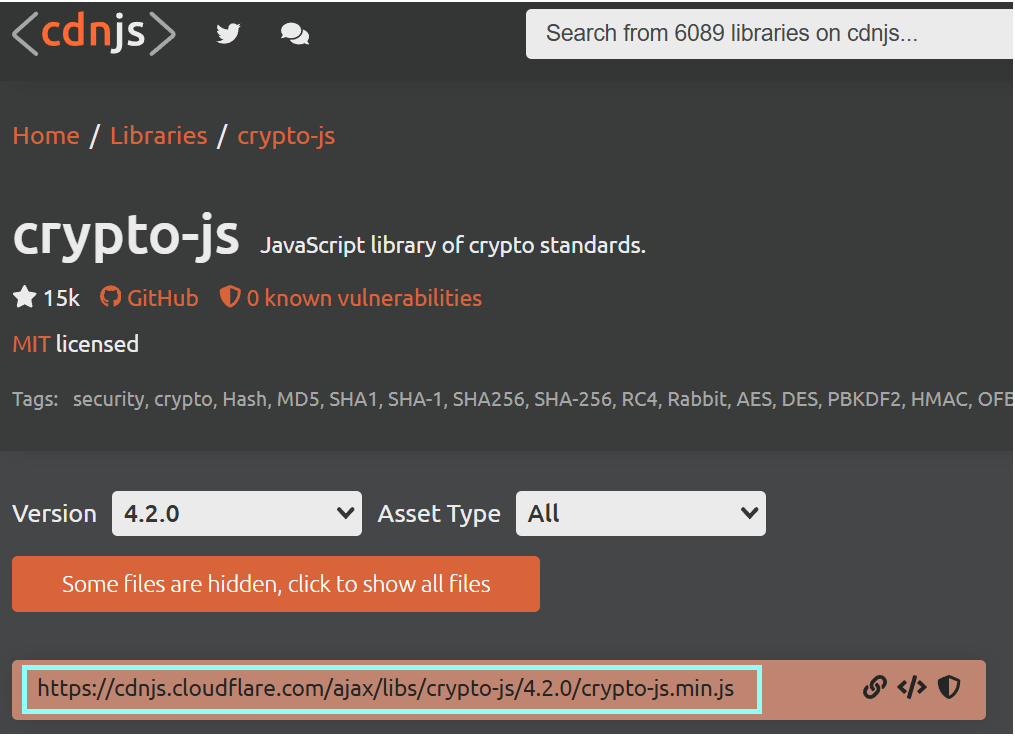
\includegraphics[width=0.8\textwidth]{Images/Parte3/4.1.png}
    \caption{Página para importar la librería de CryptoJS}
    \label{fig:libreriadeCryptoJS}
\end{figure}

Luego se debe copiar la URL que esta en el rectangulo celeste de la figura \ref{fig:libreriadeCryptoJS} y colocarlo como un ``@require'' en el código de Tampermonkey tal y como se muestra en el siguiente código \ref{code:ImportarLibreriaCryptoJS}:

\refstepcounter{codecount}\label{code:ImportarLibreriaCryptoJS}
\begin{lstlisting}[language=JavaScript, caption={Importar librería cryptoJS}]
// ==UserScript==
 ...

  // @require      https://cdnjs.cloudflare.com/ajax/libs/crypto-js/4.2.0/crypto-js.min.js
        
 ...
// ==UserScript==

\end{lstlisting}

\clearpage

\subsection{Utiliza SRI en la librería CryptoJS}

En la misma página de \href{https://cdnjs.com/libraries/crypto-js}{cdnjs} de la librería CryptoJS se puede encontrar el SRI Hash tal y como se puede apreciar en la figura \ref{fig:SRIcopiar}.


\begin{figure}[H]
    \centering
    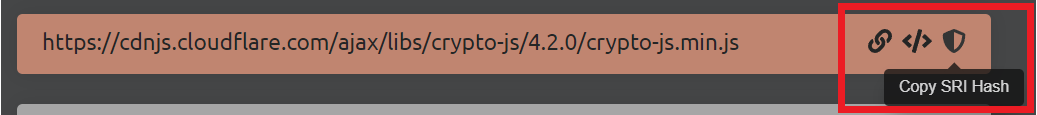
\includegraphics[width=0.8\textwidth]{Images/Parte3/4.2.png}
    \caption{SRI Hash asociado}
    \label{fig:SRIcopiar}
\end{figure}

Para utilizarlo, hay que concatenar la sentencia del código \ref{code:ImportarLibreriaCryptoJS} con el símbolo ``\#'' y luego el SRI Hash asociado como se puede ver en el fragmento de código \ref{code:SRI}

\refstepcounter{codecount}\label{code:SRI}
\begin{lstlisting}[language=JavaScript, caption={Uso de SRI en la librería CryptoJS}]
// ==UserScript==
 ...

  // @require      https://cdnjs.cloudflare.com/ajax/libs/crypto-js/4.2.0/crypto-js.min.js#sha512-a+SUDuwNzXDvz4XrIcXHuCf089/iJAoN4lmrXJg18XnduKK6YlDHNRalv4yd1N40OKI80tFidF+rqTFKGPoWFQ==

 ...
// ==UserScript==


\end{lstlisting}



\subsection{Repercusiones de SRI inválido}

Para mostrar que pasaría si se usa un SRI invalido, se copia otro SRI Hash de la página tal y como se ve en el código \ref{code:SRIINVALIDO}:

\refstepcounter{codecount}\label{code:SRIINVALIDO}
\begin{lstlisting}[language=JavaScript, caption={Uso de SRI en la librería CryptoJS}]
// ==UserScript==
 ...

  // @require      https://cdnjs.cloudflare.com/ajax/libs/crypto-js/4.2.0/aes.min.js#sha512-UOtWWEXoMk1WLeC873Gmrkb2/dZMwvN1ViM9C1mNvNmQSeXpEr8sRzXLmUSha1X4x5V892uFmEjiZzUsYiHYiw==

 ...
// ==UserScript==


\end{lstlisting}

\clearpage

Luego, al recargar la página no se logra apreciar ninguna alteración hecha por Tampermonkey. No obstante, cuando se inspecciona la consola se imprime el error ``Uncaught (in promise) TypeError: r is undefined'' tal y como se muestra en la figura \ref{fig:SRIINVALDO_}

\begin{figure}[H]
    \centering
    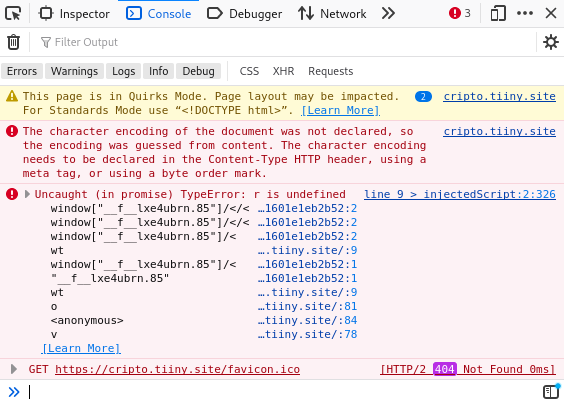
\includegraphics[width=0.8\textwidth]{Images/Parte3/4.3.png}
    \caption{Error al usar un SRI Hash invalido}
    \label{fig:SRIINVALDO_}
\end{figure}

Hay que recordar que SRI ``Subresource Integrity'' compara un hash criptográfico de un recurso externo como bien podría ser el Script que se está usando con el hash esperado de la página web. Por lo tanto, si los hashes no coinciden, el navegador bloquea estos Scripts como protocolo de seguridad por lo que es probable que este error aparezca al tratar de buscar variables que no están declaradas en la librería.

\clearpage

\subsection{Logra descifrar uno de los mensajes}

Al usar 3DES en modo ECB se puede descifrar el mensaje. Por lo tanto, a continuación se muestra en la figura \ref{fig:Devlan} la forma en la que se obtiene el mensaje descifrado mediante la página \href{https://www.devglan.com/online-tools/triple-des-encrypt-decrypt}{Devglan en éste enlace}:

\begin{figure}[H]
    \centering
    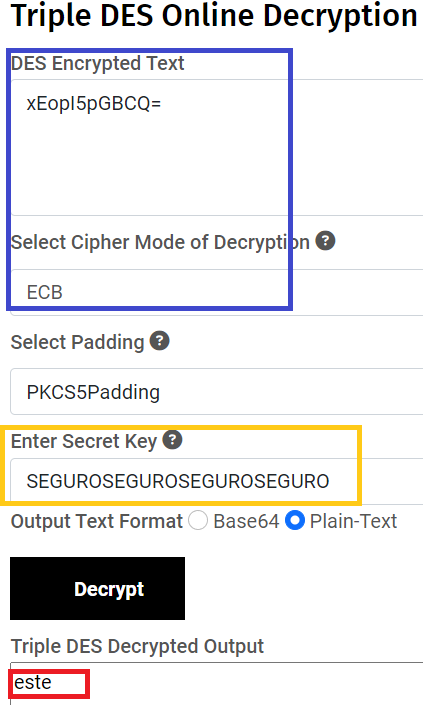
\includegraphics[width=0.5\textwidth]{Images/Parte3/4.4.png}
    \caption{Descifrado de uno de los mensajes en la página Devlan}
    \label{fig:Devlan}
\end{figure}

En esta página para descifrar un mensaje con 3DES, se tiene que:

\begin{enumerate}
    \item Rectángulo azul: Mensaje encriptado ``xEopI5pGBCQ=''.
    \item Rectángulo amarillo: La llave usada que es ``SEGUROSEGUROSEGUROSEGURO''.

    \item Rectángulo rojo: Mensaje descifrado que es ``este''
\end{enumerate}

\clearpage

\subsection{Imprime todos los mensajes por consola}

Para imprimir todos los mensajes por consola se hace uso del fragmento de código \ref{code:parte3} extraído de la página de \href{https://greasyfork.org/es/scripts/479454-cryptojs/code}{Greasy Fork}:

\refstepcounter{codecount}\label{code:parte3}
\begin{lstlisting}[language=JavaScript, caption={Mostrar mensajes en consola}]
// Parte 3
     var divs = document.getElementsByTagName('div');
     var contenidoDesencriptado = '';
     for (i = 0; i < divs.length; i++) {
         var div = divs[i];
         var id = div.id;
         var ciphertextBytes = CryptoJS.enc.Base64.parse(id);
         var decryptedBytes = CryptoJS.TripleDES.decrypt({ ciphertext: ciphertextBytes }, CryptoJS.enc.Utf8.parse(contrasena), {
             mode: CryptoJS.mode.ECB,
             padding: CryptoJS.pad.Pkcs7
         });
         var decryptedText = decryptedBytes.toString(CryptoJS.enc.Utf8);
         console.log(id + ": " + decryptedText);
         contenidoDesencriptado += decryptedText + ' ';
     }
\end{lstlisting}

Para una mayor comprensión, se procede a explicar la lógica del código \ref{code:parte3}:

\begin{enumerate}
    \item Línea 2: Se obtiene un arreglo de aquellos elementos que sean un div en su etiqueta.

    \item Línea 4: se hace un for que itera sobre cada elemento del arreglo declarado en la línea 2.

    \item Línea 5-7: se transforma el ID de string a base64 que es la codificación entendida por la librería CryptoJS.

    \item Línea 8-11: Se descifra el mensaje con decrypt en modo ECB con padding PKCS7

    \item Línea 12-13: Se transforma el mensaje descifrado a una cadena de texto y se imprime por consola.
\end{enumerate}

\clearpage

Al recargar la página, se procede a ver todos los mensajes por la consola tal y como se muestra en la figura \ref{fig:Impresiondemensajes}:

\begin{figure}[H]
    \centering
    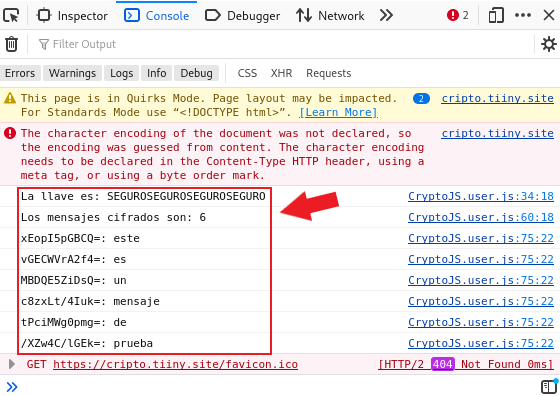
\includegraphics[width=0.9\textwidth]{Images/Parte3/4.5.png}
    \caption{Impresión de mensajes descifrados por consola}
    \label{fig:Impresiondemensajes}
\end{figure}

Los mensajes descifrados se pueden apreciar dentro del rectángulo rojo junto al cifrado correspondiente. Por otro lado, también se pueden visualizar la llave y la cantidad de mensajes mostrados en las secciones anteriores.

\clearpage

\subsection{Muestra los mensajes en texto plano en el sitio web}

Para mostrar los mensajes en texto plano, se debe concatenar el anterior código \ref{code:parte3} con el siguiente código \ref{code:parte3cont}:

\refstepcounter{codecount}\label{code:parte3cont}
\begin{lstlisting}[language=JavaScript, caption={mostrar mensajes en texto plano}]
// Parte 3
     ...
  
     var palabrasDesencriptadas = contenidoDesencriptado.split(' ');
     var mensajeDesencriptado = document.createElement('p');
     for (var k = 0; k < palabrasDesencriptadas.length; k++) {
         mensajeDesencriptado.innerHTML += palabrasDesencriptadas[k] + '<br>';
     }
  
     document.body.appendChild(mensajeDesencriptado);

\end{lstlisting}

Luego de recargar nuevamente la página, se pueden apreciar los mensajes descifrados en texto plano enmarcados por un rectángulo rojo tal y como se muestra en la figura \ref{fig:Mensajesentextoplano}

\begin{figure}[H]
    \centering
    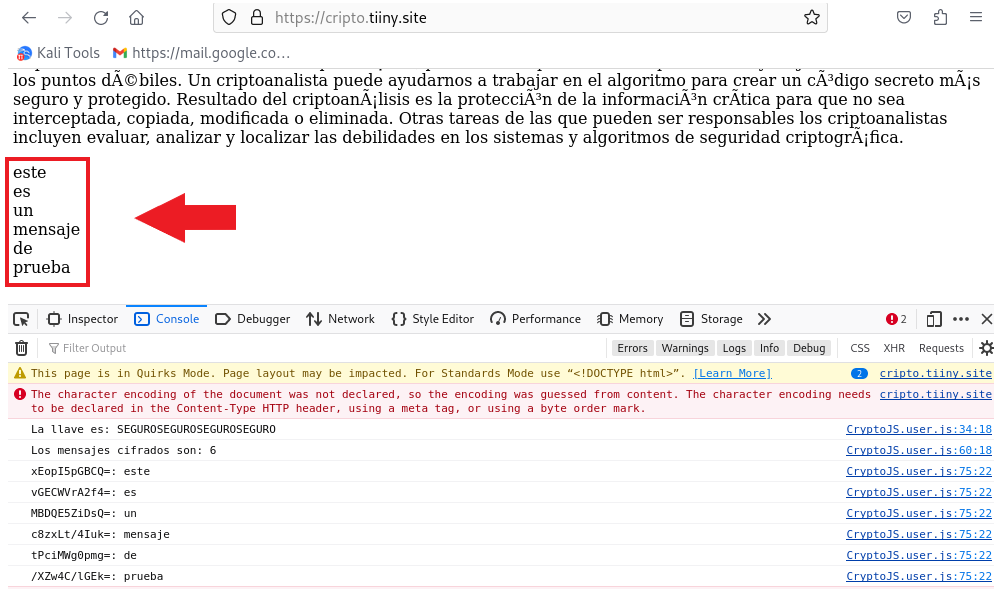
\includegraphics[width=0.9\textwidth]{Images/Parte3/4.6.png}
    \caption{Mensajes en texto plano al bajar por la página}
    \label{fig:Mensajesentextoplano}
\end{figure}

\subsection{El script logra funcionar con otro texto y otra cantidad de mensajes}

Para demostrar que el Script funciona con otro texto y otra cantidad de mensajes, se hizo una página web en react en localhost donde se muestra un mensaje distinto. Para ello se usa la página de \href{https://www.devglan.com/online-tools/triple-des-encrypt-decrypt}{devglan en este enlace} para codificar los mensajes con la llave ``CRIPTOCRIPTOCRIPTOCRIPTO'' para emular un encenario parecido al que estaba en la página del informante. A continuación se muestra en la figura \ref{fig:localhost} la página web diseñada para este caso:

\begin{figure}[H]
    \centering
    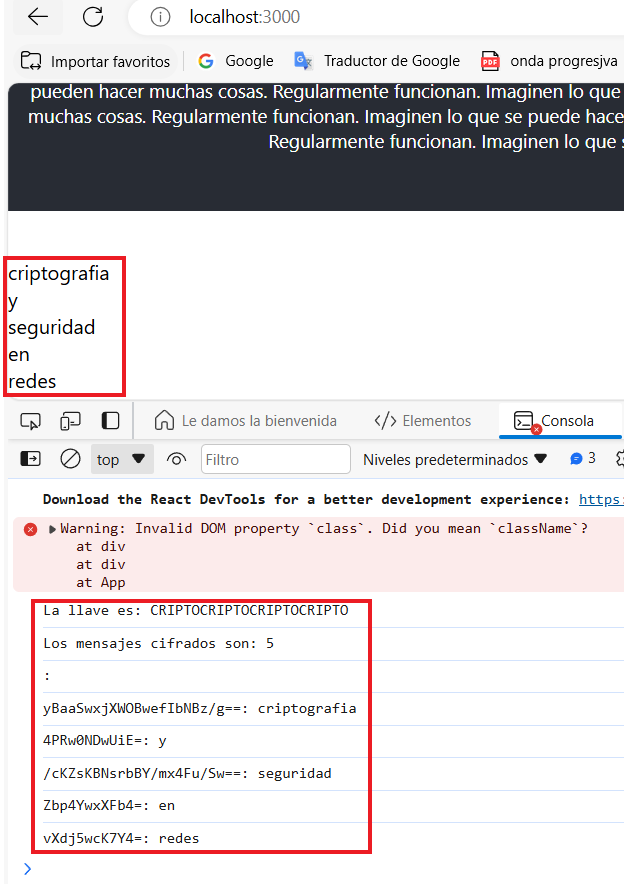
\includegraphics[width=0.67\textwidth]{Images/Parte3/4.7.png}
    \caption{Script utilizado para una página localhost mostrando un mensaje distinto}
    \label{fig:localhost}
\end{figure}

\clearpage

Tal y como se puede ver en la figura \ref{fig:localhost}, los mensajes descifrados están enmarcados en un rectángulo rojo y se puede apreciar que enlace de la pagina es localhost. Por otra parte, también se logra apreciar parte del texto que también estará en el enlace al repositorio en la sección de referencias.

\subsection{Indica url al código .js implementado para su validación}

El código pertenece al usuario \href{https://greasyfork.org/es/users/1214768-akumukernel}{AkumuKernel} de la página de  \href{https://greasyfork.org/es/scripts/479454-cryptojs/code}{Greasy Fork este enlace adjunto}. No obstante, se ha dividido el código en fragmentos para hacer las explicaciones de lo que hace cada una de sus partes y para verlo se debe acceder al siguiente \href{}{enlace a github adjunto}:

\section*{Conclusiones y comentarios}

Esta experiencia tuvo como objetivo demostrar la forma en la que se pueden enviar mensajes cifrados y ocultos mediante una página web y el uso de un Script de Tampermonkey para descifrar dichos mensajes. Cabe a destacar que Tampermonkey es una herramienta poderosa cuando se trata de alterar páginas web y es por eso que en esta experiencia se puede apreciar como lee y altera componentes de un sitio web. Por otra parte, se debe mensionar que la experiencia se hace bajo un entorno controlado, ético y con fines educativos para mejorar el servicio de protección a los datos de usuario.

\clearpage

\subsection*{Issues}

\begin{enumerate}
    \item Issue 1:

Al usar el script de Tampermonkey en modo incógnito no funciona. Entonces, para solucionar este problema, se debe ir a las configuraciones de la extensión de Tampermonkey y habilitar la opción de permitir la ejecución de dicha aplicación sobre ventanas en modo incógnito tal y como se muestra en la siguiente figura \ref{fig:Incog}

\begin{figure}[H]
    \centering
    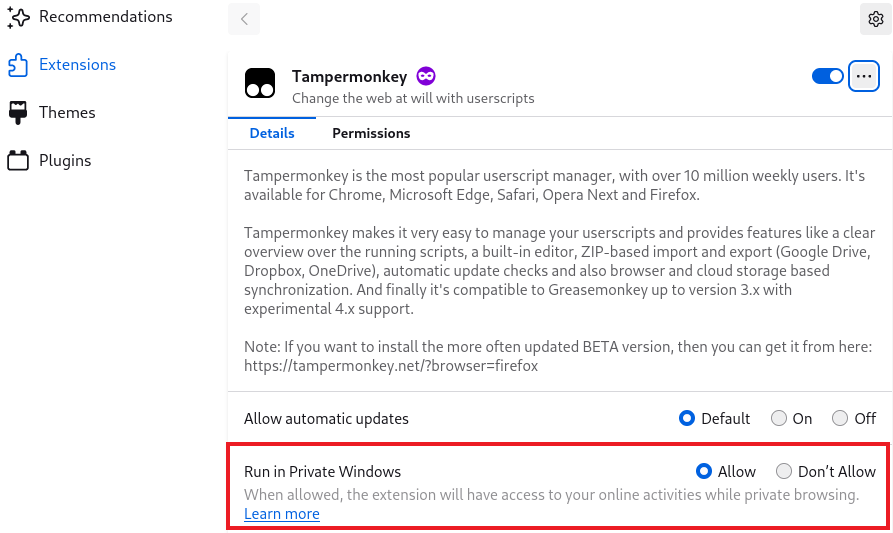
\includegraphics[width=0.9\textwidth]{Images/Issues/Incog.png}
    \caption{Solución al problema de Tampermonkey con el modo incógnito}
    \label{fig:Incog}
\end{figure}

Como se puede apreciar en la figura \ref{fig:Incog}, la opción que se debe habilitar esta enmarcada en un rectángulo rojo.

\clearpage

\item Issue 2:

Al tratar de usar la extensión en google Chrome, no funciona la extensión de Tampermonkey. Por lo tanto, para ver este problema se ha tomado un capture a la consola de la página del informante y a su vez a la configuración básica de la extensión de Tampermonkey como se puede apreciar en la figura \ref{fig:GoogleC}:

\begin{figure}[H]
    \centering
    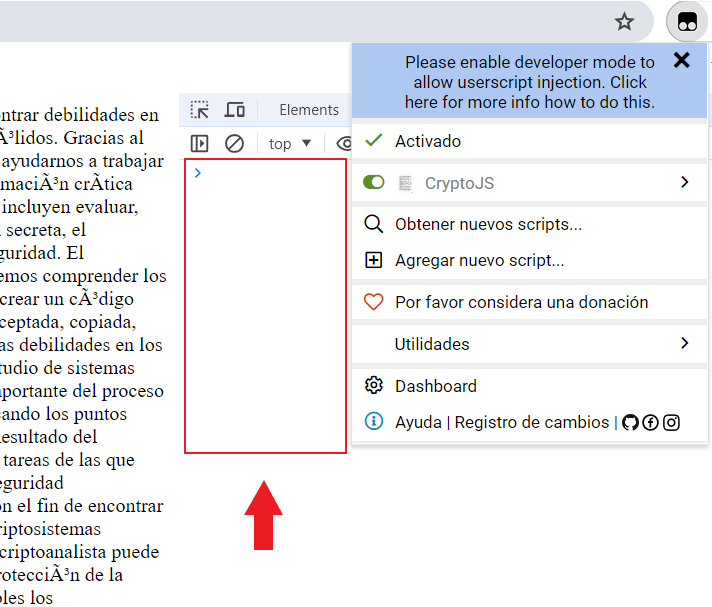
\includegraphics[width=0.9\textwidth]{Images/Issues/GoogleC.png}
    \caption{Problema al usar Tampermonkey en Google Chrome}
    \label{fig:GoogleC}
\end{figure}

Como se puede apreciar en la figura \ref{fig:GoogleC}, se ha enmarcado en un rectángulo rojo y una flecha en donde se supone que debería haber alguna impresión por consola debido a que el script de Tampermonkey esta activado. No obstante, no se muestra nada por lo que para solucionar esto, se debe de cambiar de navegador tales como Mozilla o Edge de tal forma que sea compatible Tampermonkey.

\clearpage


\item Issue 3:

Al colocar un SRI distinto, no funciona el código e imprime el error visto en la figura \ref{fig:SRIINVALDO_}. No obstante, un así existen otras opciones en la página de \href{https://cdnjs.com/libraries/crypto-js}{cdnjs} a la librería de CryptoJS tal y como se muestra en la figura \ref{fig:more}.

\begin{figure}[H]
    \centering
    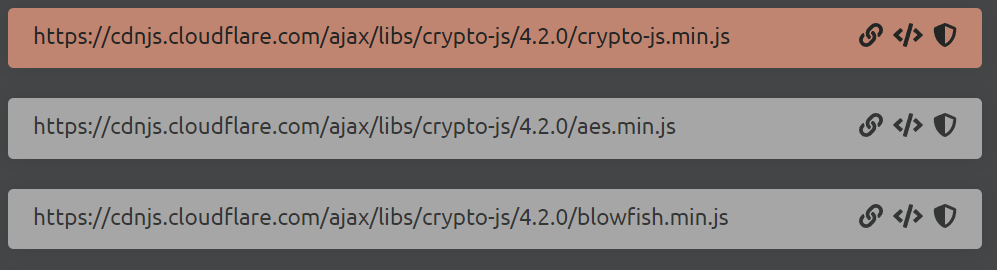
\includegraphics[width=0.9\textwidth]{Images/Issues/more.png}
    \caption{SRI distinto}
    \label{fig:more}
\end{figure}

Por otra parte, también existen distintas versiones a estas librerías por lo que cabe la duda en la forma en que se seguirán actualizando. También el hecho de que halla más librerías hace énfasis en el análisis que hace una página web para validar los recursos mediante las comparaciones que hace el SRI Hash y mantener seguro al usuario al restringir hashes que no coincidan.


\item Issue 4:

Descifrar los mensajes enviados por el informante requiere de probar distintos descifrados. Para solucionarlo se debe probar con distintos algoritmos para conseguir que el cifrado está en 3DES en modo ECB sin mencionar que tambien tenía un padding en PKCS7. Además, cuando se intentó realizar otro texto y mensaje en la sección 4.7 cabía también la posibilidad de hacerlo con otras codificaciones como bien podría ser CBC tal y como se muestra en la siguiente figura \ref{fig:more2}:

\begin{figure}[H]
    \centering
    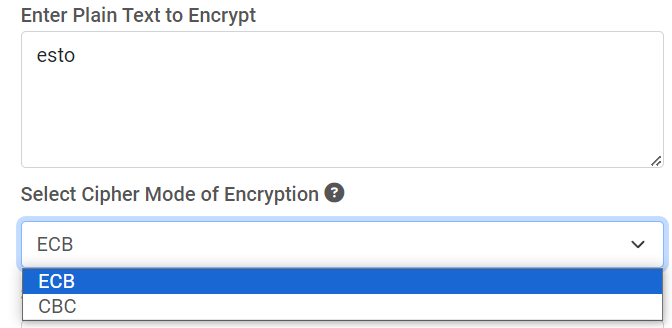
\includegraphics[width=0.9\textwidth]{Images/Issues/4.png}
    \caption{Existen más tipos de cifrados}
    \label{fig:more2}
\end{figure}

Por otra parte, se debe destacar también sirve utilizar el padding PKCS5 para descifrar los mensajes puesto a que en lo único en que difiere es en el tamaño de bloques a utilizar.



\end{enumerate}



\clearpage

\section{Referencias}

El apoyo y manejo de algunos comandos se hizo con una combinación entre el uso de herramientas de IA's de código generativas como Chatgpt y Microsoft Bing. Además, se hace uso de los códigos de los siguientes enlaces:



\begin{itemize}
    \item Página para importar la librería de CryptoJS \href{https://cdnjs.com/libraries/crypto-js}{acá}.

    \item Código de Tampermonkey del usuario AkumuKernel para descifrar la página del informante \href{https://greasyfork.org/es/scripts/479454-cryptojs/code}{acá}.

    \item Página de devglan para descifrar los mensajes \href{https://www.devglan.com/online-tools/triple-des-encrypt-decrypt}{acá}.
    


\end{itemize}


\end{document}
